\documentclass[twocolumn,10pt]{article}

\usepackage[a4paper,hmargin=1.5cm,vmargin=2.5cm,]{geometry}
\setlength{\columnsep}{0.7cm}
\usepackage{palatino}
\usepackage{graphicx}
\usepackage[utf8]{inputenc}
\usepackage{hyperref}
\usepackage{minted}
\usepackage{balance}
\usepackage{dblfloatfix}  
\usemintedstyle{colorful}
\usepackage[font=small,labelfont=bf]{caption}
\urlstyle{same} % no tt font for URLs
\newcommand{\blockade}{\rule{3em}{0.7em}}  %% Marker for things to change before submission

\usepackage{natbib}
\bibliographystyle{genome_research}
\setcitestyle{aysep={}} 

\usepackage[dvipsnames]{xcolor}
\hypersetup{
    colorlinks,
    linkcolor={blue!50!black},
    citecolor={blue!50!black},
    urlcolor={blue!50!black}
}
\renewcommand{\dbltopfraction}{0.7}
\renewcommand{\textfraction}{0.2}

\begin{document}

\setcounter{secnumdepth}{0}


\twocolumn[{%
\centering
\textbf{\Large R/LinkedCharts: A novel approach for simple but powerful interactive data analysis}
\vspace{1.5ex}

Svetlana Ovchinnikova and Simon Anders\\
{\footnotesize Center for Molecular Biology of the University of Heidelberg, Germany}
\vspace{1.5ex}

24 January 2020
\vspace{6ex}
}]

\section{Abstract}
In exploratory data analysis, one usually jumps back and forth between visualizations that provide overview of the whole data and others that dive into details. In data quality assessment, for example, it might be very helpful to have one chart showing a summary statistic for all samples, and clicking on one of the data points would display details on this sample in a second plot. Setting up such interactively linked charts is usually cumbersome and time-consuming to use them in \emph{ad hoc} analysis. We present R/LinkedCharts, a framework  that renders this tasks radically simple: Producing linked charts is as quickly done as is producing conventional static plots in R, requiring a data scientist to write only very few lines of simple R code to obtain complex and general visualization. We expect that the convenience of our new tool will enable data scientists and bioinformaticians to perform much deeper and more thorough EDA with much less effort. Furthermore, R/LinkedCharts apps, typically first written as quick-and-dirty hacks, can also be polished to provide interactive data access in publication quality, thus contributing to open science.

\section{Introduction}

The problem of effective visualization has been there since the first reported experiment results \citep{friendly_2001}. The continuously growing amount and complexity of available data over the last decades made it a challenging issue \citep{fisher_2017}. For a while, the only possible way to tackle the problem was to develop more elaborate types of plots employing colour, shape, transparency, and other visual aspects to combine multiple layers of information \citep{keahey_2013, bertin_2011, heer_2009}. Yet, there are certain limits to how much information one can learn from a static image \citep{hegarty_2011}. Excessive details and multiple overlapping layers make it harder to grasp the crux of a plot. Thus, a researcher has to decide what information to keep and what to dismiss to convey the message better\citep{odonoghue_2018}. It is, doubtless, an essential step since data often contain a lot of noise and information irrelevant to the point one tries to make. Yet, it may be useful to provide the reader with a way to estimate the relevance of the omitted piece of data on his or her own to avoid biases \citep{bresciani_2009} and boost confidence in reported data patterns.

With the advance of modern technologies, interactive visualization emerged to offer new ways of presenting information \citep{newman_1979, becker_1987}.(It's been there since whatever...) In an interactive figure, there is no need to fix all the parameters or to exclude any data that do not contribute to the main idea. Instead, the user gets a chance to experiment with data and details quickly and intuitively, concentrating at once on the plot's most exciting or suspicious parts. Numerous tools \citep{caldarola_2017} now provide means of creating interactive visualizations not only for research \citep{noronha_2017, wick_2015, hillje_2020, broman_2015} but also for any area that involves data analysis and presentation of any kind \citep{zhao_2012, wu_2010}. Alongside apps for a specific task, one can also find low-level grammars \citep{bostock_2011, satyanarayan_2015}, and more high-level but still generally purposed packages \citep{satyanarayan_2016, shiny, p_2019, sievert_2019, sievert_2020}.

The advantage of interactivity lies beyond just simplifying navigation through big or complex data. When it takes just a click or two to add changes to a plot, it urges a researcher not to put aside ideas or concerns and thus go through the data more thoroughly. At the same time, readers can check conclusions and claims of a paper on the fly, without going through all the script and analysis, thus making the findings more credible. Therefore, we believe that further integration of interactive tools in a researchers' routine can significantly improve the quality of studies \citep{shander_2016, yuk_2014}.


Today many authors accompany their papers with an interactive resource to present their data and results \citep{travaglini_2020, roider_2020, kalucka_2020}. Though these visualizations are often useful and provide a comprehensive insight into the data, they generally serve presentation and communication purposes. Only after the most work on the project is finished, researches spend a couple of days deploying a fancy interactive app to share their data and results with the scientific community \citep{batch_2017}. We, however, believe, that interactivity should become a part of everyday routine to facilitate data exploration. To this end, the tool to produce interactive apps should be both simple and highly customizable.

\begin{figure*}[b]
	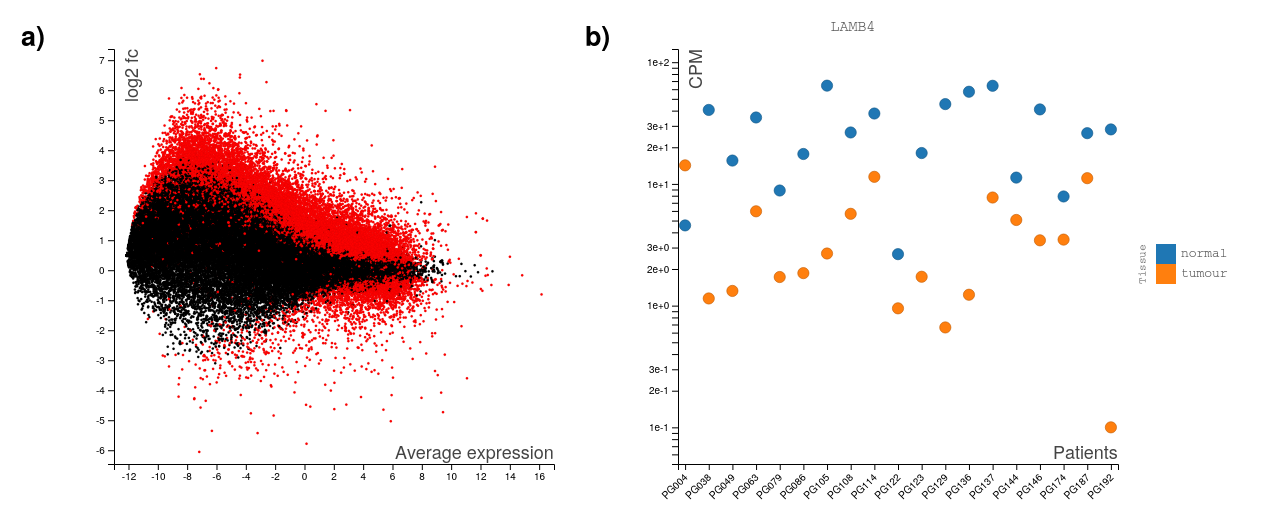
\includegraphics[width=\textwidth]{FigD/figD.png}
	\caption{Overview of genes differentially expressed in cancerous and normal tissues from \citet{conway_2015}. MA-plot (a) shows all the sequenced genes with their average expression on X-axis and log-fold change on Y-axis. Red indicates genes, where the difference was reported as significant by the ``limma''  \citep{ritchie_2015}  package. Plot to the left (b) shows expression values (CPMs) for a selected gene (in this case, LAMB4) and all the patients. This figure is based on a LinkedCharts app, and its live version is provided in the supplement. When the user clicks on a point of the MA-plot, the expression plot changes, showing the new selected gene. In such a way, one can check immediately, whether the genes, labeled as significantly different, are interesting for further study.}
	\label{FigD}
\end{figure*}

Simplicity should serve as an incentive to use interactivity whenever there is any smallest hint that it may be useful. If a tool is too complicated, one may prefer to do most of the analysis by more habitual static means, and wait for a special occasion when it is worthwhile to invest time and effort into an interactive app. It should also be similar in design to most common visualization means since tools with too specific interface tend to be used by people with more extensive programming skill. Even if a researcher with less expertise in coding has an eager-to-help colleague, he or she may be unwilling to ask for assistance in petty everyday tasks and wait for something big.

Still, an attempt to simplify a tool may end in hardcoding and presetting too many parameters. As a result, a simple-to-use tool can require a particular data structure and be fit only for precise data flow patterns. And any attempt of going beyond in-built limitations, if at all possible, can cost a considerable effort. It is not necessarily a disadvantage, since much of routine work in the lab involves typical for the area steps and data types. Yet, it may be useful if one does not try to force a research problem in the predefined mould but instead makes the visualization tool fit the given task. For that, a reasonable degree of flexibility is required.

With the LinkedCharts, we tried to find a balance between the two goals of a tool for interactive data exploration. It requires only basic coding skills to produce fully functional apps for \emph{ad hoc} analysis. With a little more effort, one can make a nicer looking app and customize most commonly used plot settings (such as colours, labels, axes, etc.). And finally, with the time and effort generally required for the same task with other packages, one can use LinkedCharts to make a presentable app deployed on a server. Since the library is JavaScript-based, it can be combined with various existing web solutions. One can also write custom scripts that will change even hardcoded aspects of the library without making changes to the source code, making LinkedCharts extremely flexible. 

LinkedCharts is not fixed on any specific task. It is a toolbox, and its blocks can be combined in any manner the same way as one combines plots for a complex paper figure. All blocks share the same interface and very similar interactivity capabilities, which means that understanding one of them is enough to grasp the entire concept of LinkedCharts.

With all these, we hope that LinkedCharts can become a useful asset for a scientific community that can be used both for everyday routine and for presenting one's research to a greater audience. LinkedCharts available as an R package (``rlc'', can be downloaded from CRAN) and as a JavaScript library. This paper's focus is on R implementation of LinkedCharts, which we also refer to as R/LinkedCharts. 

\section{Results}

\subsection{Linking charts}

\begin{figure*}[t]
	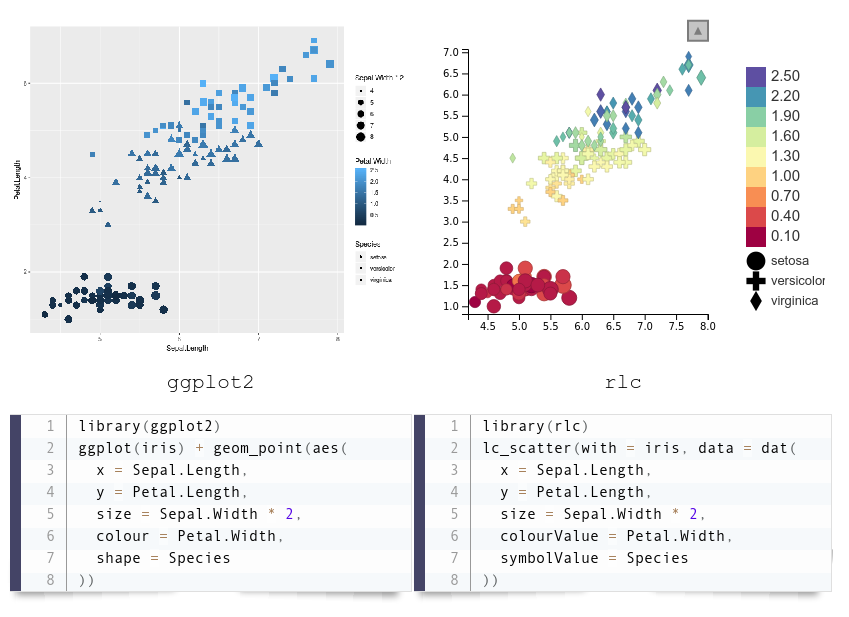
\includegraphics[width=\textwidth]{FigB/figB.png}
	\caption{Typical syntax of an R/LinkedCharts plot and its comparison with the ``ggplot2'' \citep{wickham_2016} package as an example of one of the most commonly used plotting libraries. Lines of code are arranged to put the same aspects of the charts next to each other. ``iris'' dataset, which is one of the R built-in datasets, was used for this example. Both pieces of code are fully functional, and their output is shown above the code.}
	\label{FigB}
\end{figure*}

The central concept behind LinkedCharts is, as follows from the name, linking and focusing \citep{buja_1991}. We connect two to or more plots so that manipulations with one of them affect the others. It is easier to understand how this concept works in LinkedCharts with a simple example based on data from \citet{conway_2015}.

In this study, three samples were taken from 17 patients with oral cancer: Of normal, cancerous, and dysplasia tissues. mRNA from all these samples was sequenced to obtain gene expression values. The first natural question to ask based on these data is about differential expression between various tissues. Several packages offer functionality to answer such questions  \citep{ritchie_2015, love_2014}. Here, we have applied function \mintinline{R}{voom} from the ``limma'' package to compare normal and cancerous tissues. It is common to visualize such a comparison with an MA-plot \citep{dudoit_2002} showing the average gene expression on the x-axis and log fold change between the two groups on the y-axis (Fig \ref{FigD} (a)). Red dots correspond to genes that are considered significantly different between the two conditions (adjusted p.value < 0.1). But how does the difference in expression look like for every single patient? Is it persistent across all the patients or only detected in some of them? Are there any artefacts or outliers that cause the p.value to be too small?

To find answers to these questions, we can add another plot that shows expression values (CPMs) for all the patients (Fig \ref{FigD}(b)). This plot can show expression for only one selected gene at a time, but LinkedCharts allows one to link it to the MA-plot. Now, any click on a point from the MA-plot makes the plot to the right show expression of the corresponding gene. Fig \ref{FigD} is based on the LinkedCharts app, which is provided in this paper's supplement. We encourage the reader to pause for a moment and check it to get a feeling of LinkedCharts. There, we also provide full code to generate the app and links to necessary data files to immediately get this app in one's R session and experiment with it. For this and all further examples, we provide two versions of code: minimal with only essential parameters needed to make app functional, and more extended with custom colours, labels, etc. In the paper, we only focus on the minimal code.

To further explore the linking mechanism, we can look at the code that generates the app from Fig \ref{FigD}. It is a minimal, but full code for the app. For now, we concentrate only on the highlighted lines.

\begin{figure*}[b]
	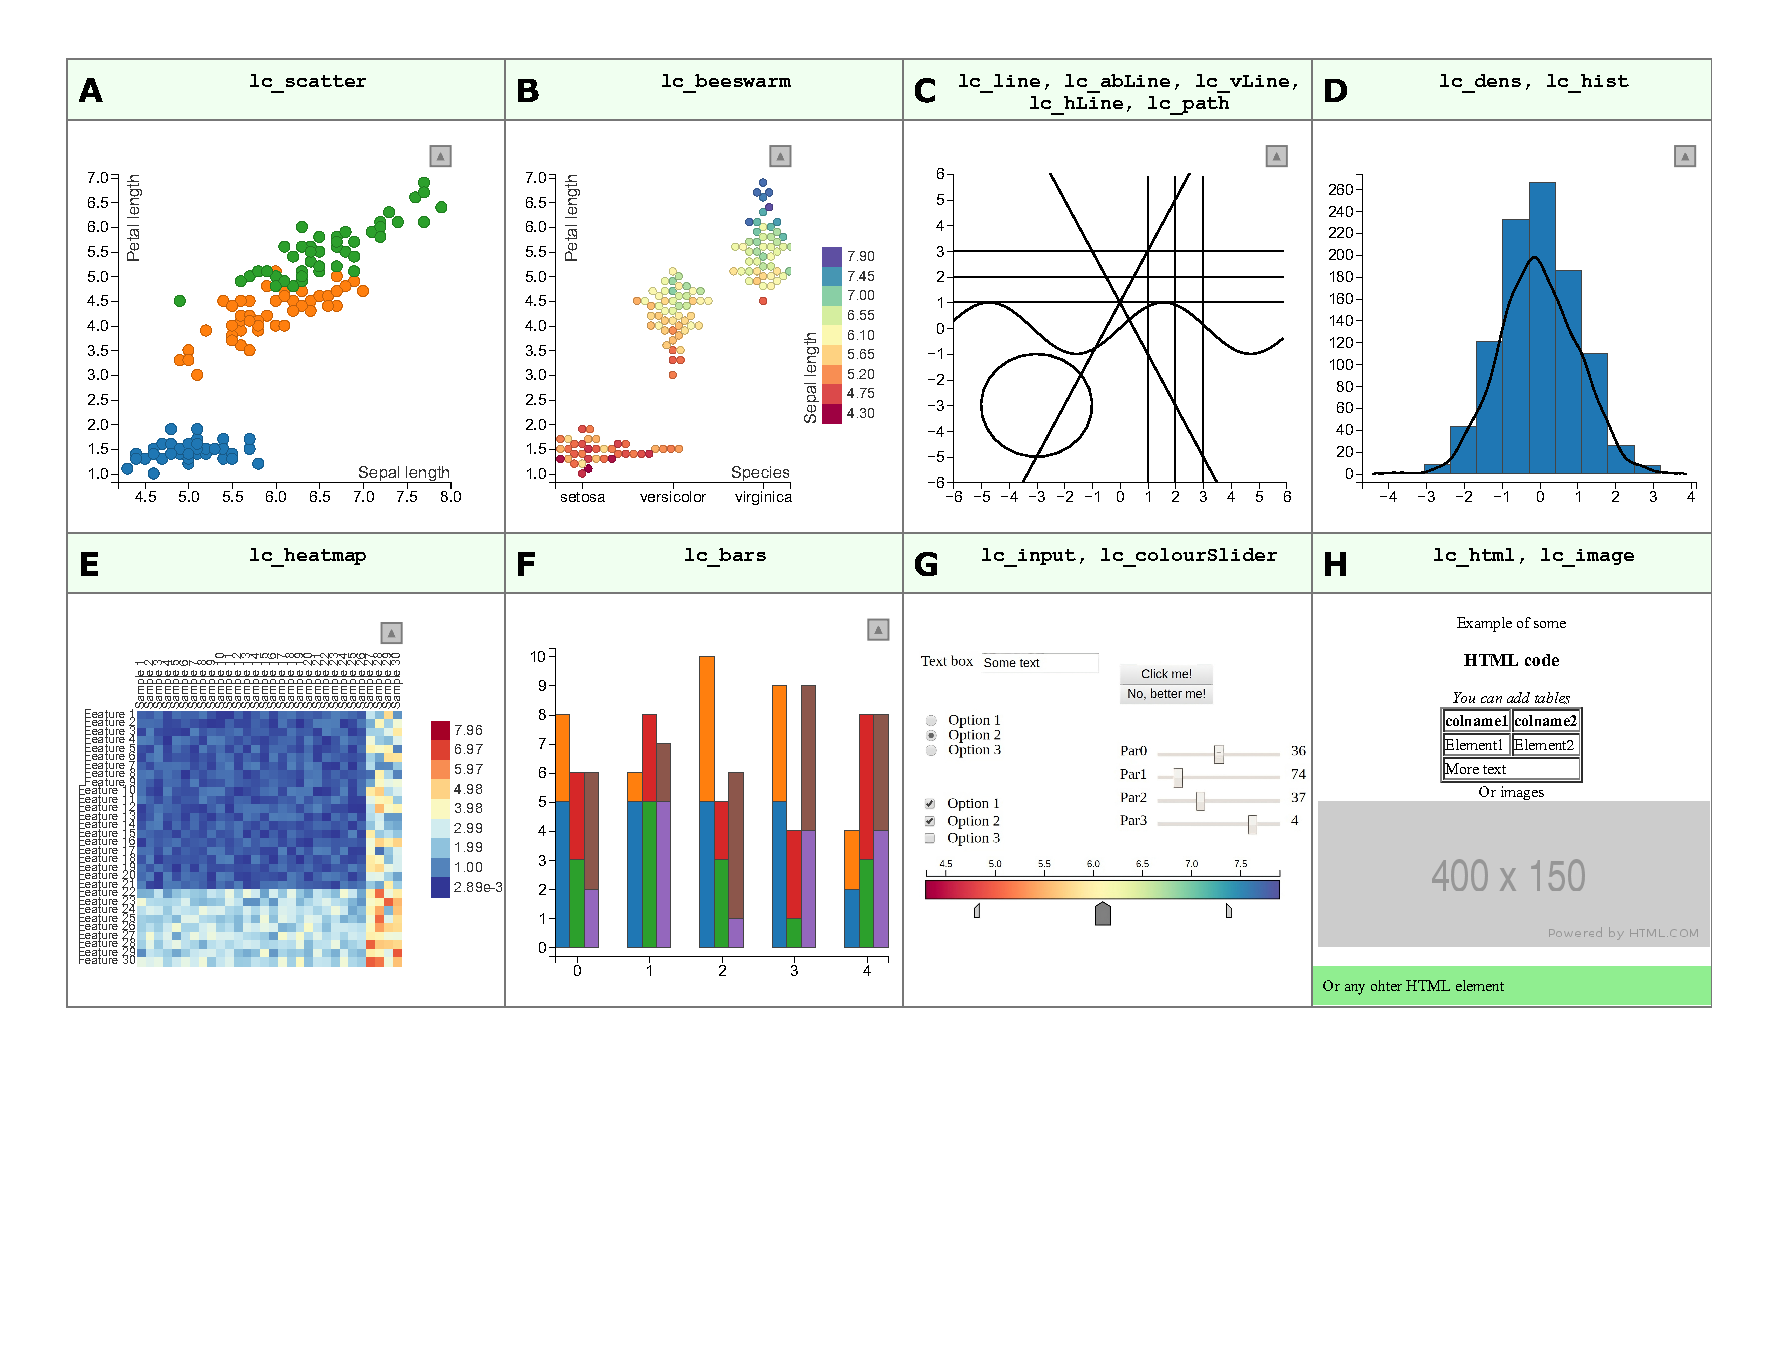
\includegraphics[width=\textwidth]{FigA/figA.png}
	\caption{Gallery of all available plotting functions the in ``rlc'' package. A scatter plot (a); a bee swarm plot (based on d3-beeswarm plugin \citep{lebeau_2017}) (b); a collection of various lines (c); a histogram and a density plot (density was multiplied by a factor of 500 to be visible on the same plot as the histogram) (d); a heatmap (e); a bar chart (f); a collection of interactive elements to gather input from the user (g); functions to add custom HTML code and static plots to the page (h). All these examples with code to create them can be found in the supplement.}
	\label{FigA}
\end{figure*}

\begin{minted}[highlightlines={2,9-12,17}]{R}
openPage(layout = "table1x2")
gene <- 1

lc_scatter(dat(
   x = AveExpr,
   y = tissuetumour,
   colour = ifelse(adj.P.Val < 0.1, 
                   "red", "black"),
   on_click = function(k) {
      gene <<- k
      updateCharts("A2")
   }),
"A1", with = voomResult)

lc_scatter(dat(
   x = patient,
   y = normCounts[gene, ],
   colourValue = tissue, 
   logScaleY = 10),
"A2", with = sampleTable)
\end{minted}

It works as follows. In the \mintinline{R}{gene} variable, we keep an index of the gene to show in the expression plot. This index is used to tell the chart, which line of the \mintinline{R}{normCounts} matrix (it is where normalized counts are stored) to use as y values of the plot: \mintinline{R}{y = normCounts[gene, ]}. Almost every chart of the R/LinkedCharts library has the \mintinline{R}{on_click} argument, which is a function, that will be called each time the user clicks on an element of the plot (point, line, cell of a heatmap, etc.). In this example, whenever it happens, we change the value of \mintinline{R}{gene} to the clicked point index. Then we tell R/LinkedCharts to update the second plot (``A2'' is its ID set in the last line of the example). Updating means that the package will reevaluate all arguments inside the \mintinline{R}{dat()} function and change the chart accordingly. In our case, a new value of \mintinline{R}{gene} will yield new y values for the expression plot.

This simple logic is not limited to just two plots and provides a base to create various simple and complex apps. For example, one of our tutorials (\url{https://anders-biostat.github.io/linked-charts/rlc/tutorials/citeseq1.html}) gives detailed instructions to generate an app for single-cell data exploration. The app consists of four charts, three of which are scatter plots and one is an information table to show genes that define a selected cell cluster.

Besides a click, LinkedCharts can react to other events, such as moving the mouse over or out of an element, selecting or deselecting elements with the \emph{Shift} key pressed, clicking on any position of a plot or on a heatmap label. The full list can be found on a man page for any function of the ``rlc'' package. Understanding how to define these functions (above is shown a very typical example) is everything one needs to generate apps that run locally. More profound knowledge is required only to deploy an R/LinkedCharts app on a server. 

\subsection{Basic syntax}

Overall, we tried to make R/LinkedCharts simple and recognizable by any user with a fundamental knowledge of R. Any chart has a set of properties to define each of its specific aspects. One can already notice this from the previous example, where vectors of values were used as x and y coordinates of points or their colours. The same principle works in most plotting libraries. For example, Figure \ref{FigB} shows a comparison of syntax in R/LinkedCharts (``rlc'' package) and ggplot (``ggplot2'' \citep{wickham_2016} package) for a simple scatter plot. Lines are arranged to match the same aspects of the plots; there is its output above each code block. One can see that the input data structure is identical, and there is hardly any difference between the two.

An important thing to notice here is the \mintinline{R}{dat()} function. One can set properties in the same manner both inside and outside of it, but only those that are inside the \mintinline{R}{dat()} function will be evaluated on each call of \mintinline{R}{updateCharts}. Everything outside this function will remain constant. There is a small example that can illustrate the effect of the \mintinline{R}{dat()} function.

\begin{minted}{R}
lc_scatter(
   dat(x = rnorm(30)),
   y = rnorm(30))
\end{minted}

Running this code will produce a scatter plot with 30 randomly located points. Now, every time one calls \mintinline{R}{updateCharts()} x coordinates of each dot will change to a new random value, but all the y coordinates will remain the same.

So far we have mentioned only scatter plots, but R/LinkedCharts is not limited to them. There are 15 main functions in the ``rlc'' package. Each generates a specific type of plot (such as scatter plot, heatmap, bar plot, etc.) or a navigation element (such as sliders or text fields). Figure \ref{FigA} shows them all together with some basic examples. Each plot, as it has been already mentioned, is defined by its properties: some of them are required (such as \mintinline{R}{x} and \mintinline{R}{y} for a scatter plot or \mintinline{R}{value} for a heatmap) many others are optional (\mintinline{R}{palette}, \mintinline{R}{title}, \mintinline{R}{ticks} etc.). A full list of all the properties with live examples is available at \url{https://anders-biostat.github.io/linked-charts/rlc/tutorials/props.html} and also on the R man page for each plotting function. Many of the properties accept minor variations in spelling (\mintinline{R}{colour/color} or \mintinline{R}{labels/label}).

\subsection{Use Cases}
\subsubsection{Quality check}

Generalising data is of great importance in any research project that concerns big data. It is troublesome to see patterns and make meaningful conclusions from raw readouts and measurements. Researches routinely count aligned mRNA reads, select only informative features, calculate various scores, etc. An appropriate generalisation is a key to uncovering biological patterns hidden in the data, but it also means loss of information.

Figure \ref{FigD} nicely illustrates the process. To see the overall difference between the tissue types defined by thousands of genes, we make an MA-plot. It immediately tells us that there is a big difference between the tissue types, noticeably more genes with higher expression levels in the cancerous tissue and that the difference in downregulated genes in tumour samples seems to be more pronounced. All that we get by representing the original 38 expression values (dysplasia samples not included) per sample for each gene with just three: average expression, logarithmised fold change in expression between normal and cancerous tissues, and the significance estimate of this difference. Such a generalisation allowed us to see the bigger picture but at the cost of individual expression values.

A similar approach is a part of almost any pipeline used in a biological study. Each step takes the output from the previous one and modifies it, usually by generalising it to produce more interpretable data. However, some information is inevitably put aside. And from the resulting picture alone, it is hard, if not impossible, to see whether the raw data had any problems that could influence further conclusions. Various quality checks are devised to detect any possible issues with the omitted data. They are often quite helpful in pointing the researcher's attention towards some spurious artefacts in the data. Yet, especially in studies involving big data, these checks are fully automated. The researcher only looks at some summarised reports and may also have a look at some random examples. If those look reasonable, the general assumption is that all the data not filtered out is valid. However, while there is only one way for everything to be correct, there are numerous ways for the data to be either wrong or not as one has expected. Therefore, it's essential to have a possibility to look back before making any conclusions from a figure that shows a condensed result.

This idea is the primary motivation behind the LinkedCharts library. Figure \ref{FigC} demonstrates it. If we have a workflow or a pipeline that performs certain transformations of the data, LinkedCharts offers an easy way to look back through each of the steps. Whenever a researcher encounters an interesting or suspicious pattern in the data, he or she can, with minimal effort, check whether it is a real biological finding or some technical artefact missed by quality checks. 

\begin{figure*}
  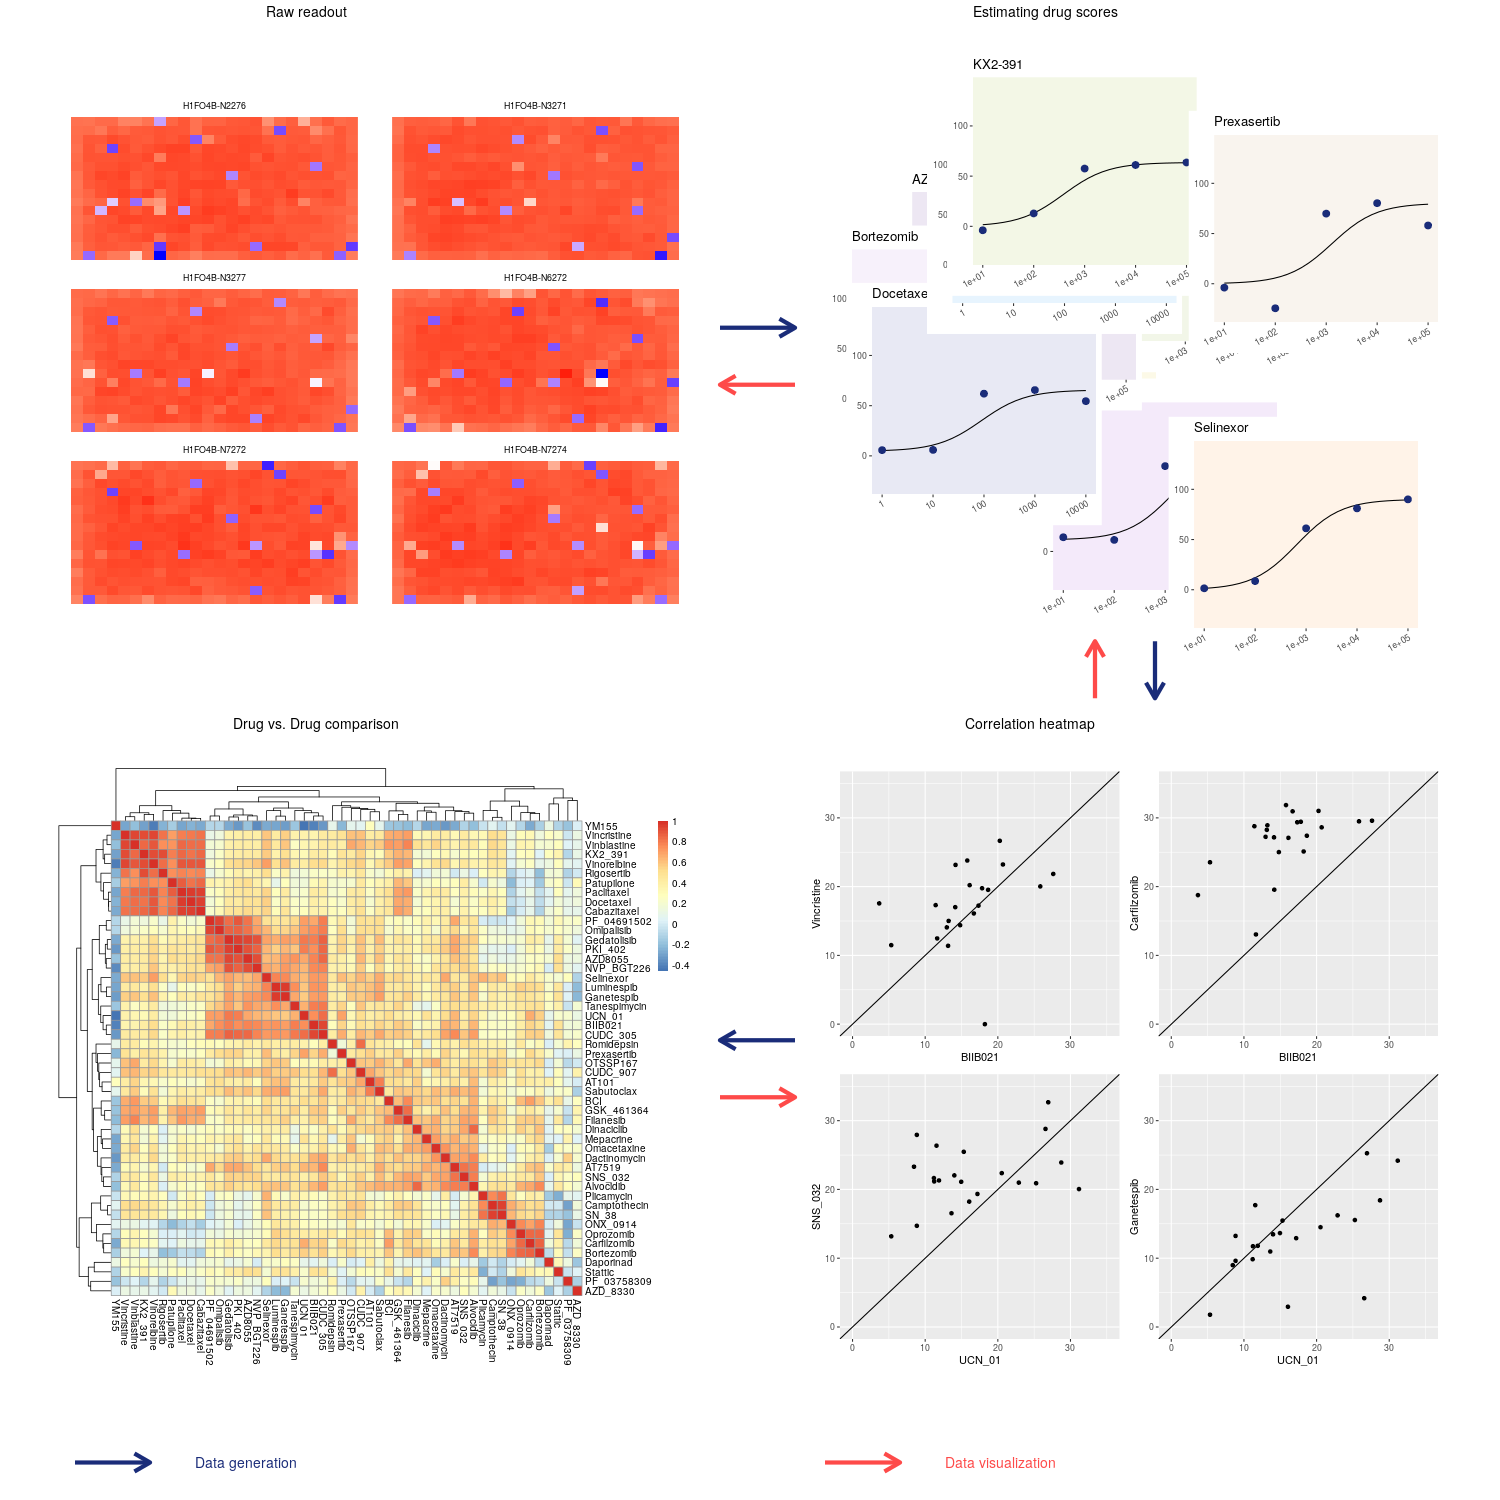
\includegraphics[width=\textwidth]{FigC/figC.png}
  \caption{Main idea behind the LinkedCharts library is shown based on a drug screening experiment. The blue arrow shows the direction of a common pipeline used in drug screening experiments. We start with reading intensity values from plates with different cell lines grown in the presence of studied drugs in different concentrations (A). These values are then normalised and aggregated to yield a single score for each drug (B). Different drugs' scores are compared to each other across all the tested cell lines (C). A drug-drug correlation heatmap is then produced to identify clusters of similar drugs (D). Red arrows illustrate visualisation direction. We start by showing the summary heatmap plot (D). If the researcher is interested in a particular cell or a cluster of cells, he or she can examine the corresponding drug scores simply by clicking on the cell (C). Similarly, one can examine the exact viability values for any given drug (B). And finally, if needed, it's possible to take one more step back and to look at raw readouts to inspect them for the presence of any artefacts (A)}
  \label{FigC}
\end{figure*}

R/LinkedCharts is particularly useful in generating chains of ``linked'' plots, where each chart explains an element of the previous one. We presented one of the simplest examples in the ``Linking charts'' section as a basic R/LinkedCharts app. Figure \ref{FigC} shows another one with a longer chain, which is also available in the supplement. It is based on the data from \citet{he_2018}.

For demonstration purposes, we use only a subset of data to simulate a typical drug screening pipeline. In this subset, 50 drugs in five different concentrations were tested against 17 pancreatic cancer cell lines. The main heatmap shows drug-drug correlation values. By clicking on a cell of the heatmap, the user selects two drugs and can check individual drug scores for each of them against all the tested cell lines. The inhibition values were calculated based on drug activity in five tested concentrations. So the third plot shows all those activity levels for each concentration. Finally, one can also find raw readouts from the plates to check for plate-related effects, if any. In this manner, each chart represents one of the major steps of the pipeline that led from plate readouts to a correlation heatmap to identify clusters of drugs with similar behavioural patterns. One can find more details as well as code and links to download the data in the supplement. 

Such apps would allow a quick and easy spot check of uncovered data patterns and give the researcher a better understanding of inner connections between the data. For instance, to what extent noise can influence the signal or what scale of changes in the value of interest is typical to the data.

\subsubsection{Exploratory analysis}

While interactivity is already increasingly used to present results of finished studies to the research community, with R/LinkedCharts, we would like to point out its usefulness for everyday exploratory analysis. To this end, R/LinkedCharts is designed in a way that requires one to spend not more time designing an app than it would take to perform a similar analysis with static plots. One may think of R/LinkedCharts as a container where the researcher can put their code to turn it into an interactive app. It will not perform a complex analysis automatically, but it will also not ask for much more than the usual routine coding, one should do with or without interactivity. Basic yet custom and functional apps do not require any special knowledge of ``rlc'' underlying structure or HTML layout. With this, we have attempted to encourage researchers to try out interactivity as a more improvised and need-based approach.

Let us return to the example from Figure \ref{FigD}. There we showed a typical part of a differential expression study: an MA-plot (Figure \ref{FigD}A) and a plot with expression values for each sample to explore it (Figure \ref{FigD}B). We have already shown in Figure \ref{FigB} (section ``Basic Syntax'') that making a static plot in R/LinkedCharts is not much different in comparison to popular plotting libraries. It will take the same effort and same data structuring and preprocessing to make these plots with, for example, the ``ggplot2'' library, as with the ``rlc''. Now, the plot in Figure \ref{FigD}B serves for spot-checking. It allows one to dive into the details of expression patterns, but only for one gene at a time. Of course, one may decide to only rely on the general overview that is provided by the MA-Plot (Figure \ref{FigD}A). However, a better practice is to make sure that there are no unexpected expression artefacts in the genes of interest. To do that, one would usually try to get a list of genes to check by filtering, using some special R tools, or somehow else, and then make a plot like the one in Figure \ref{FigD}A for each of them.

In the most simple case it would take copying and pasting the code for the spot check plot and replacing \mintinline{R}{y = normCounts["MyGene", ]} with \mintinline{R}{y = normCounts["AnotherMyGene", ]} (see the code chunk in the section ``Linking Charts''). A little improvement to that would be to write \mintinline{R}{y = normCounts[myGene, ]} and keep updating the \mintinline{R}{myGene} variable: \mintinline{R}{myGene <- "MyGene"}, then \mintinline{R}{myGene <- "AnotherMyGene"}. After each update one should stil copy a piece of code that generates the plot into the console. Finally, the most effective way is to place this constantly copied and pasted code into a function, let say, \mintinline{R}{makePlot} and to call it, when necessary: \mintinline{R}{makePlot("MyGene")}, then \mintinline{R}{makePlot("AnotherMyGene")}.

Now, we kindly ask the reader to pause here and return to the section ``Linking Charts'', where the code to produce the app from Figure \ref{FigD} is given. The \mintinline{R}{onClick} function does the same thing that is described in the previous paragraph. It stores the new gene into the variable \mintinline{R}{k}. It then performs an equivalent of copying and pasting to the console the code for the second plot, which in the ``rlc'' library can be done with just the \mintinline{R}{updateCharts} function for the sake of simplicity. The core idea here is so identical to the usual spot-checking routine that one can add our imaginary \mintinline{R}{makePlot} function to the ``rlc'' chart, and it will still work. It is only essential to be aware that in this case, the argument to the \mintinline{R}{makePlot} will be an index of the selected gene and not its name.

Thus, there are simply no additional requirements to the data or environment, no practices that one should adopt to perform the usual exploratory analysis or even to convert an existing script into an interactive app. Figure \ref{FigE} shows such a transformation in details for another example of a common spot check practice.

\begin{figure*}[t]
  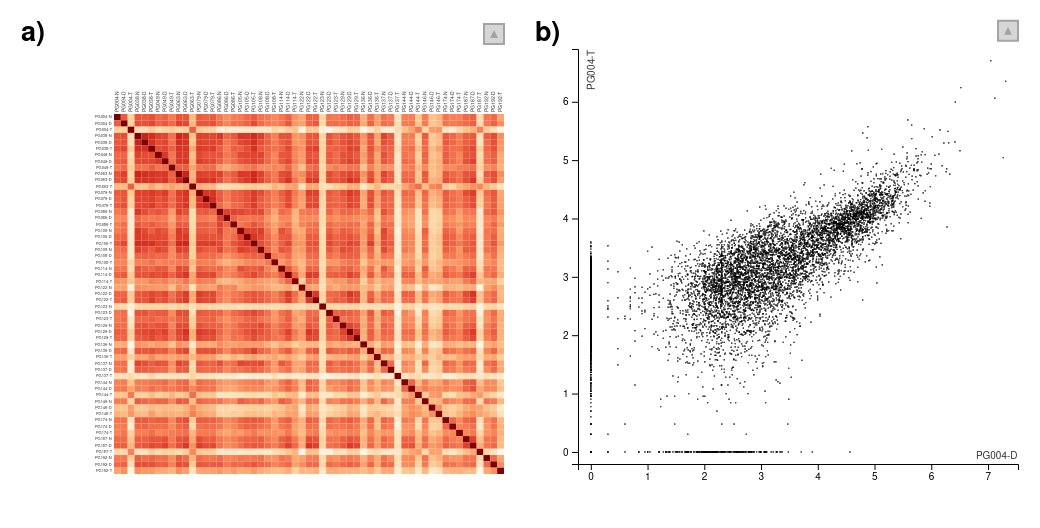
\includegraphics[width=\textwidth]{FigE/figE.png}
  \caption{ Example of an R/LinkedCharts app (c, d) that can be used during exploratory analysis and the code to generate it in comparison with the static plots (a, b) for the same purpose. The heatmaps (a, c) show Spearman correlation of gene expression for all samples from \citet{conway_2015}. Here, we can see two clear outliers in each heatmap's right and bottom and some more or less pronounced clusters of samples with similar gene expression levels. The scatter plots (b, d) show expression values for two samples plotted against each other. Browsing through several such plots can help the researcher get a feeling of the data and explore unexpected patterns like the outliers mentioned above. The code is split into two pieces, where the upper one is responsible for generating the ``static'' plots (in the case of ``rlc'' charts, they are still interactive, just not linked), the lower part shows the code to update them. For static plots, one has to execute the same lines of code for any pair of samples he or she wants to compare, while for R/LinkedCharts the provided code should be added to the list of arguments for the heatmap. After that, switching between pairs of samples is done simply by clicking on the corresponding cell of the heatmap. The static heatmap (a) was generated with the ``pheatmap'' package; scatter plot (b) was made with a base R function. The live version of the app can be found in supplementary. For simplicity, gene expression for all the samples is subsetted to 8000 randomly selected genes.}
  \label{FigE}
\end{figure*}

This example is also based on the oral cancer data \citep{conway_2015}. Above, we have looked at differentially expressed genes between normal and cancerous tissues. Still, before getting there, a researcher who has just obtained these data may want to get some overview of the samples. One of the common ways to do so is to check how well the samples correlate with each other by making a correlation heatmap (Figure \ref{FigE}A and \ref{FigE}C). It can immediately show us if the samples from the same patient are more or less similar to each other than those of the same type, and it can also highlight possible outliers. In Figure \ref{FigE}(A, C), one can easily spot two of such outliers: the two samples to the right and bottom that are further from their nearest neighbours than most samples are from the majority of all others. The next most natural question to ask is how exactly these two samples are different from others. To answer it, one can plot gene expression values for several pairs of samples against each other (Figure \ref{FigE}B and \ref{FigE}D). It will give us a feeling of what ``similar'' means for the particular dataset and how the outliers do not fit this pattern. Therefore, the visualisation task at hand reminds the one described above and illustrated by Figure \ref{FigD}. Figure \ref{FigE} shows how to solve this problem with commonly used static plots (a heatmpam from the ``pheatmap'' \citep{kolde_2019} package and a base R scatter plot, Figure \ref{FigE}AB) and with R/LinkedCharts (Figure \ref{FigE}CD). Below each set of charts, there is the code necessary to generate and update them. Neither the output nor the required commands are much different between the two. However, the R/LinkedCharts app is interactive and, besides linking, provides other useful features such as zooming in and out, reclustering heatmap and showing sample names when the mouse is hovering above them.

This similarity makes R/LinkedCharts a helpful tool for exploration. The required effort to produce an interactive app is the same as to make traditional static plots. The only significant difference in the coding style that the user needs to get used to is to update one of the plots with a custom function and not by copying and pasting the same piece of code. However, such an approach is usually considered a better practice. In addition, the on-the-fly draft apps that were used for exploratory analysis can later be combined into a more complex app to present final results without a need to start from scratch.

\begin{figure*}[t]
   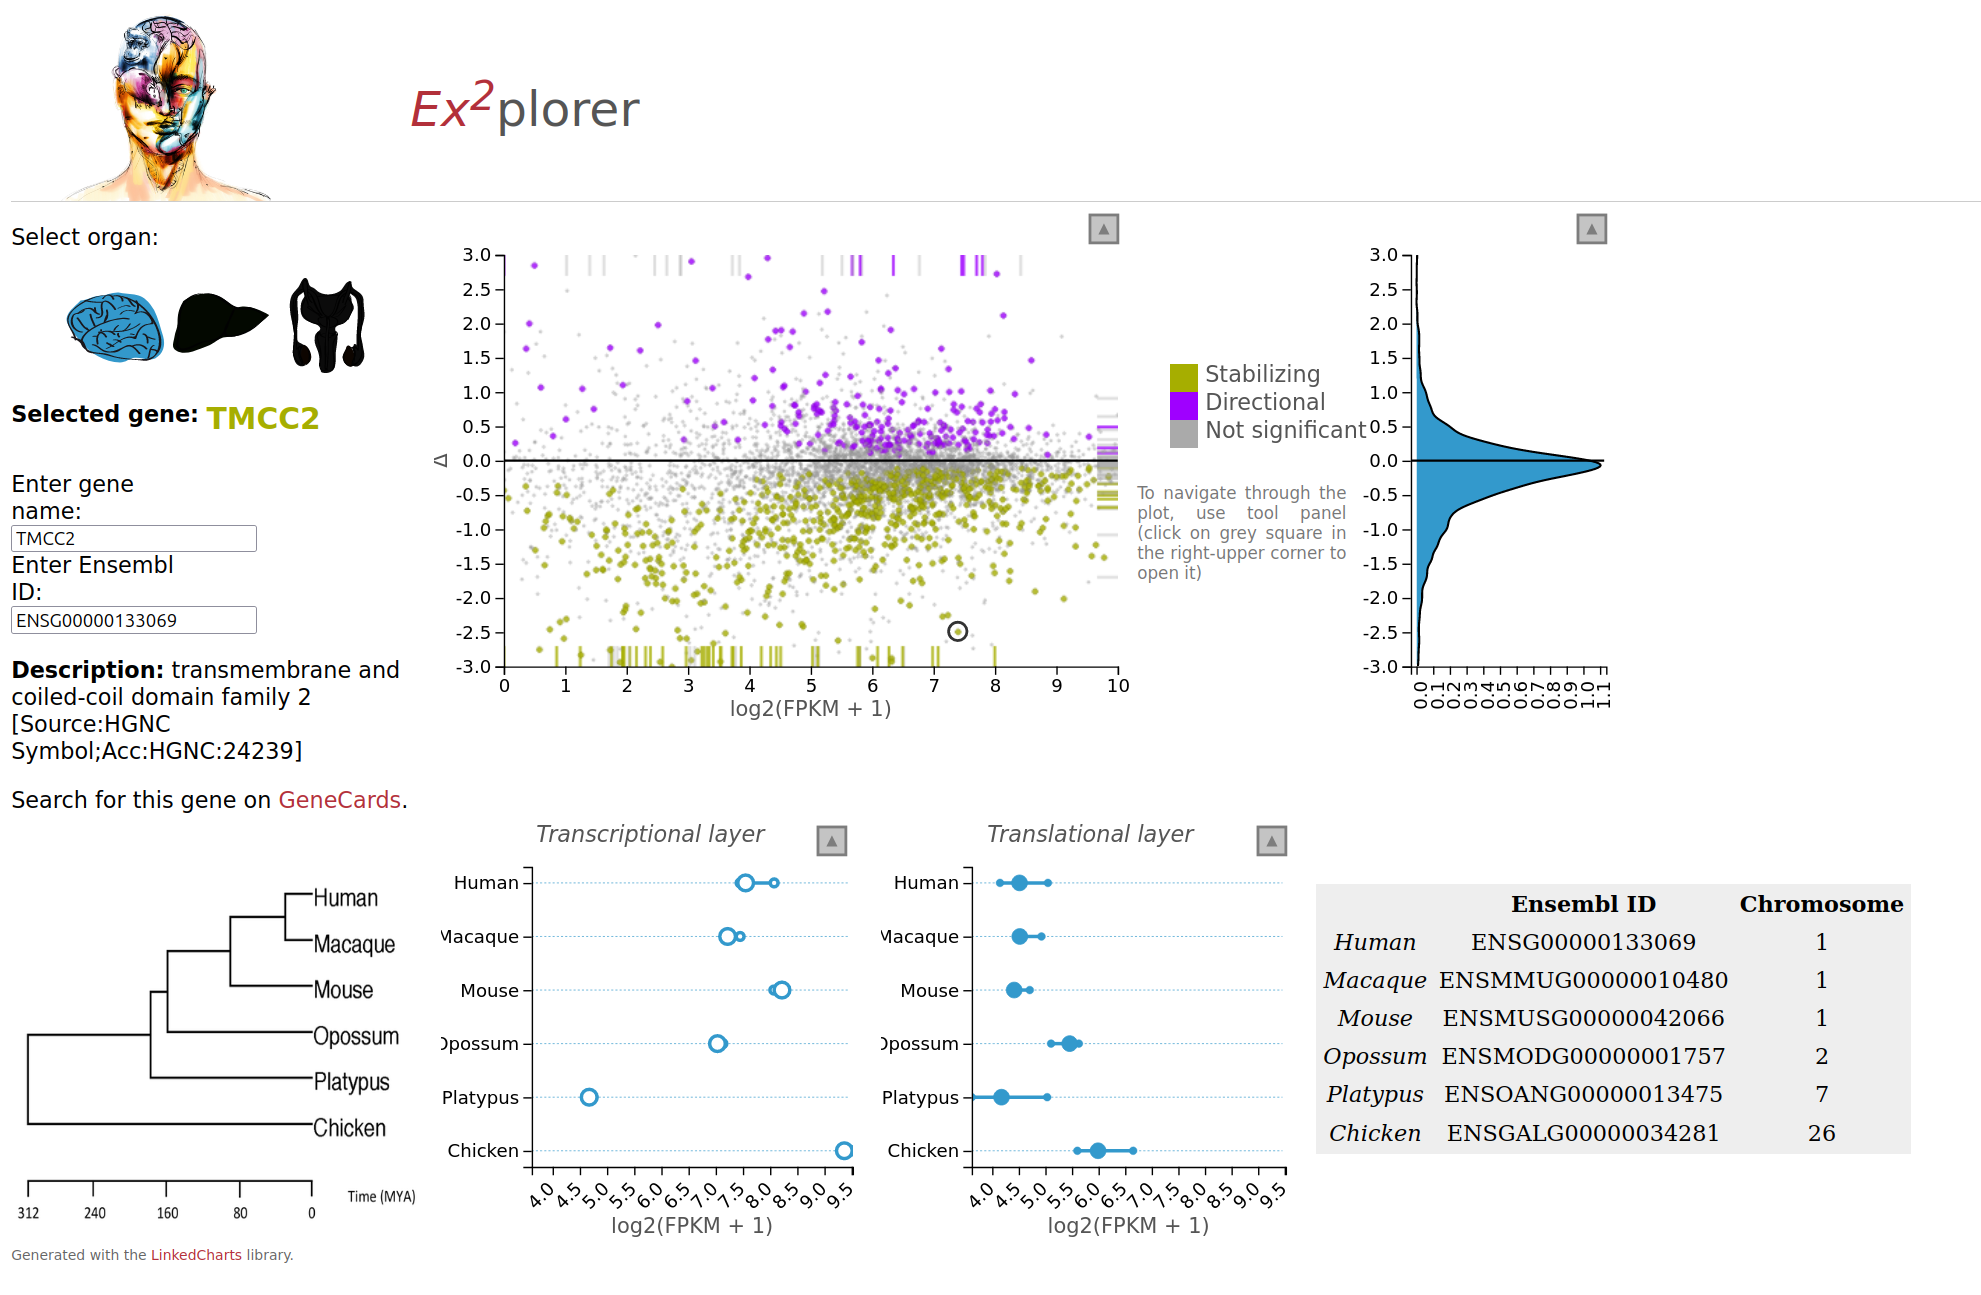
\includegraphics[width=\textwidth]{FigF/figF.png}
   \caption{An example of a stand-alone app with LinkedCharts. The app was used as a supplement for \citet{wang_2020}}
   \label{FigF}
\end{figure*}

\subsubsection{Server apps}

Any R/LinkedCharts app starts a server that listens to a given or randomly chosen port. To any request for the start page, this server answers with all the charts the user has added so far. In practice, it means that multiple users can access any R/LinkedCharts app if they can send a request to the server. It does not require any additional parameters to be set. Any of the examples we have shown in different sections of this paper can be deployed on a server. Then, multiple users can access these apps, but their sessions will not be independent.

For the complete functionality, there is one more thing that has to be set. In a LinkedCharts app, one or several ``state'' variables are used. These are generally global variables that store currently selected genes, samples, etc. and are changed inside callback functions: \mintinline{R}{gene} from the example in the section ``Linking charts'', \mintinline{R}{xSample} and \mintinline{R}{ySample} from the example in Figure \ref{FigE}. If several users are using these apps simultaneously, each click will change the state variables and consequently change the current state of charts for all the users. It can nevertheless be useful if, for example, several people are using the app as a visual addition to an online meeting. Still, in most cases, one would like interactivity to be independent for each user.

To this end, one needs only to enumerate state variables within the \mintinline{R}{openPage} function and give them some default values. For instance, the example from Figure \ref{FigE} can be turned into a server app simply by adding the following line in the beginning.

\begin{minted}{R}
openPage(sessionVars = list(xSample = 1, ySample = 2))
\end{minted}

Now, multiple users can work with the app.

Of course, there are other settings to customise a server app. In addition to the charts, one can specify other default content for the page or scripts to be run for each new user. R/LinkedCharts provides tools to control each client session: for example, to close inactive for specified time sessions, limit memory usage or the number of active connections simultaneously. Still, all these parameters are optional. More information about possible options can be found on R man pages for classes \mintinline{R}{App} and \mintinline{R}{Session} of our ``jrc'' package.

\subsubsection{Stand-alone apps}

Any app made with R/LinkedCharts (``rlc'' package) requires a connection to a running R session. However, it is only responsible for sending required data to the app, while all the visualisation and interactivity handling happens on the JavaScript side. This fact makes it possible to use LinkedCharts for generating stand-alone apps in the form of an HTML page. Such a page can then be sent to a collaborator or used as a supplement file for a paper. Unlike a link to an app deployed somewhere on a server, this kind of interactive supplement will be available to any user with an installed web browser at any moment, without a need for the research team to maintain a running app on the server. A supplement to this paper is an example of such an app contained within an HTML page. Another app was made for \citet{wang_2020}. A screenshot of this app is shown in Figure \ref{FigF}.

To make such an app, one has to be familiar with JavaScript syntax and basic concepts. The extensive knowledge may only be required to perform complicated calculations directly in JavaScipt or define complex reactions to interactive events. LinkCharts provides R and JavaScript packages (``rlc'' and linked-charts.js), and both are based on the same principles. Because of this similarity, the conversion for simple apps is pretty straightforward. Every chart property turns from an argument of a plotting function into a method of the corresponding chart object. In most cases, neither property name nor input requirements changes, but callback functions to define property values are recommended for smoother interactivity. To get a feeling of these changes, one can look at the supplement to this paper. There, every example is provided together with R code and its equivalent in JavaScript.

The most complicated part of LinkedCharts stand-alone apps is loading the data. Due to security reasons, JavaScript in a browser cannot access local files without the user explicitly uploading them. That makes data input quite tricky, despite a variety of existing parsers for most commonly used formats. The easiest way for an R user to solve this problem is to convert data into JSON format and directly insert it into the JavaScript code. JavaScript can then interpret the data as an array or an object. There are also other ways of loading data into a JS/LinkedCharts app, described in our tutorial \url{https://anders-biostat.github.io/linked-charts/js/tutorials/data.html}. Also, on this web page, one can find more tutorials and examples for a JavaScript part of the LinkedCharts library.

Unfortunately, we can not provide users with an automated converter of R/LinkendCharts apps into their JavaScript counterparts. Unrestricted customisation is an essential part of the ``rlc'' package. We want to provide researchers with a way to wrap any scientific ideas into an interactive app rather than fit the problem into a preset pattern. To this end, we do not limit user by a predefined set of callbacks, strict rules for data structuring or any other manipulations with the app. From a running R session, the user gets truly complete control over the app. Therefore, for reliable transformation of an ``rlc'' app into an HTML file, one needs a converter of R language to JavaScript, which, to our knowledge, does not exist.

\subsection{Further customization}

Since LinkedCharts is JavaScript-based, it can be combined with many existing web solutions without changing the source code of the package. One can customise the charts' appearance with CSS, add additional scripts, specify an HTML layout. R/LinkedCharts can add interactive charts to an existing HTML page supplied as \mintinline{R}{startPage} argument of the \mintinline{R}{openPage}. Additional images, files or scripts can be loaded from a directory specified by the \mintinline{R}{rootDirectory} argument. Moreover, the ``jrc'' package (available on CRAN) on top of which ``rlc'' is built allows one to run any JavaScript code directly from your R session. All this gives the user full control of what the app looks like and how it functions. Therefore a LinkedCharts app can be fitted to the specific needs of the particular project.

\section{Discussion}

Interactivity has already proved itself to be useful for data visualisation. Static plots can accommodate only a limited number of accents. Any change, no matter how small, requires one to make a new plot. And yet, it is important to look at the data from different angles and on different scales both to find peculiar patterns and to make sure that there are no hidden artefacts that can influence conclusions. Sometimes, even the visualised transition from one state to another is what helps to understand the data. Thus interactive visualisation is helpful during the research and for presenting data to the scientific community.

The field of interactive visualisation is an actively developing one with some already well known and established tools such as ``shiny'' \citep{shiny} or ``plotly''\citep{sievert_2020}. Yet, possible benefits of interactivity are far from being explored. We have described LinkedCharts as a library for spontaneous and highly customiseable visualisation. Simple interface makes R/LinkedCharts suitable for generating minor on-the-fly apps for data exploration. It can be used by researchers with only basic experience in R or by bioinformatians who are not are not willing to invest much time into an acquaintance with an unfamiliar visualisation library. The linking mechanism is ensured by user-defined callback functions, which allows R/LinkedCharts to do without requirements for fixed data structuring. There are no restrictions on the linking scheme. Every chart can be linked to any other or to multiple ones, any kind of backwards or partial linking is also possible.

We believe easy exploratory analysis to be the main niche for R/Linked charts. As we showed, it provides users with a possibility to generate visualisations with the same effort as one generally puts into a routine data digging and exploration. However, interactive apps are much more engaging than the static plots that are commonly used on the early stages of any project. When checking an idea or concern takes just a click, the researcher is more likely to thoroughly go through the data and with this, maybe, save time on the further steps of the analysis.

Once the need to present final or intermediate results to colleagues arises, the same basic apps that were previously used as ``quick and dirty'' solutions can be prettified and shared by deploying the app on a server. The required changes for a R/LinkedCharts app to work on the server are minimal, and therefore there is no need to start from scratch. One can utilise the same scripts as personal drafts for exploration and as a basis for result presentation.

LinkedCharts is a JavaScript based library, and unlike in existing alternatives we gave users full freedom to employ the functionality of various web solutions. For example, R/LinkedCharts can be embedded into any predefined HTML layout. Therefore, someone with experience in web design may provide the researcher with a custom HTML page with allocated containers for the chart and any predefined functionality that is made available by hundreds of JavaScript packages developed specifically to ensure user's interaction with a web page. Moreover, the ``jrc'' package on top of which R/LinkedCharts is built, allows to run any JavaScript code from the R session and any R code from the web page with that providing endless possibilities for custom functionality and design. Such an app can also load locally stored scripts, images, stylesheets, etc.

The JavaScript basis of R/LinkedCharts offers an interface of its own that is also very simple and similar to the ``rlc'' syntax. This gives a user who is familiar with JavaScript or willing to learn its essentials a way to convert R app into a stand-alone one that is fully contained within an HTML page. Such an app doesn't require any side resources, can be shared by email between collaborators and opened in any browser. It does not need to have a constantly running R session and can be published on any hosting including the most simple ones that does not allow to run other software in the background. An example of such stand-alone apps is the supplement to this paper. There one can also find an examples of conversion from R apps to JavaScript ones. More information can be found in our online tutorials.

The structure of JS/LinkedCharts library and even principles of JavaScript as a language to manipulate DOM elements can allow an experienced user to customise not just the ecosystem in which LinkedCharts will be embedded but the charts themselves without a need to dive into the source code. One can go as far, as defining custom types of charts (see \url{https://anders-biostat.github.io/linked-charts/js/tutorials/layers.html} for more details on that).

Overall, R/LinkedCharts serves two main purposes to facilitate data exploration and presentation. It offers an easy way to utilise interactivity for every day research tasks. And it also provides user with a possibility to fully employ the power of JavaScript for presenting the data. The later aspect addresses more experienced users and thus has no limits for possible customisation of a LinkedCharts app.


\subsection{Implementation}

R/LinkedCharts is a JavaScript visualization library with R-based \citep{R_2019} interface. The JavaScipt part is build on top of D3 \citep{bostock_2011} and the user-interface is provided by the ``jrc'' package \citep{jrc_2020}, which in turn heavily relies on the ``httpuv'' \citep{cheng_2020} package.


\begin{small} 
\balance
\bibliography{lc}
\end{small}

\end{document}


